\chapter{Частицы, волны и энергия разрешения}

\section{Частицы или поля?}

О чём физика элементарных частиц? О частицах---но этот ответ сразу же ставит древний вопрос. Дискретность здесь означает, что вещество состоит из отдельных, неделимых единиц, а не то, что оно тактично. Греческое слово \emph{atom} означает «неделимый», хотя объекты, которые теперь называют атомами, можно расщепить. Пока \emph{particle} будет общим названием для дискретной единицы.

Противоположная картина — континуум. Тогда вещество — не совокупность отдельных кусочков, а непрерывно размазанное по пространству распределение. Её естественный язык — язык полей. Поле — это функция положения: плотность вещества есть поле, и электрическое и магнитное поля — тоже поля. Последние определяют, как движутся заряженные частицы, но сами поля в классическом представлении мыслятся как непрерывно распределённые в пространстве.

Исторический порядок этих идей не следует понимать слишком буквально. Эта последовательность полезна потому, что показывает логику рассуждения, а не потому, что даёт надёжную хронологию. Лексика частиц включает атомы, молекулы, столкновения и локализованные объекты; лексика континуума включает поля и непрерывно меняющиеся свойства. Какое представление верно? Квантовая механика не позволяет ни одному из них быть полностью верным, но и не позволяет ни одному из них быть полностью неверным.

Изложение будет отчасти самодостаточным, хотя дальнейшие рассуждения опираются на квантовую механику, классическую механику, специальную теорию относительности и электромагнетизм. Непосредственный вопрос пока проще: что впервые убедило людей в том, что вещество действительно дискретно?

\section{Химические свидетельства дискретности вещества}

Первые серьёзные свидетельства появились, по крайней мере в этом логическом изложении, скорее из химии, чем из физики. Это различие искусственно: химия в значительной мере есть физика атомов и молекул. Дальтон сравнивал массы одинакового числа молекул разных веществ. Установить, что образцы содержат одинаковое число молекул, само по себе было большой проблемой. Здесь появляется имя Авогадро, и моль — это число Авогадро молекул. Само численное значение этого числа не требовалось, если нужно было лишь сравнить образцы, содержащие одинаковое число молекул.

Поразительная закономерность состояла в том, что молярные массы оказывались приблизительно целыми кратными молярной массе водорода. Множители, как правило, были не \(3/2\), не \(\pi\) и не произвольными действительными числами, а числами, близкими к целым. Например, углерод-12 содержит примерно двенадцать единиц массы, заданных водородом. Это сильно наводит на мысль о построении из повторяющихся блоков почти одной и той же массы.

Современное объяснение снимает эту загадочность. Обычные атомы содержат протоны, нейтроны и электроны. Масса электрона составляет лишь примерно одну двухтысячную массы протона или нейтрона, поэтому вклад электронов в атомную массу мал. На протоны и нейтроны приходится почти вся она, а их массы отличаются намного меньше, чем на один процент. Поскольку ядро обычного водорода — это один протон, масса атома или молекулы приблизительно является целым кратным ядерной массе, характерной для водорода. Это утверждение лишь приблизительно: массы протона и нейтрона не тождественны, и электроны тоже вносят небольшой вклад. Тем не менее почти целочисленная закономерность выявляет дискретные составляющие.

Затем молекулы стали понимать как комбинации атомов. Химия XIX века выделила примерно сто видов атомов и организовала их в элементы; если считать только элементы, примерно девяносто два из них встречаются в природе, а при учёте изотопов появляются дальнейшие различия. Периодическая таблица не периодична в наивном смысле простого повторения одинаковых блоков, но она упорядочила эти отдельные виды. На том этапе сами элементы выглядели элементарными строительными блоками. Работа Эйнштейна 1905 года дала количественный способ установить молекулярную теорию вещества гораздо более убедительно, но химические свидетельства уже сделали атомную картину убедительной.

Ближе к концу девятнадцатого века эта кажущаяся конечная точка оказалась не окончательной. Был открыт электрон, а радиоактивность выявила явления, которые картина, в которой элементы считались элементарными, не могла охватить. В радиоактивности уже в миниатюре содержались многие вопросы, из которых выросли ядерная физика и физика элементарных частиц.

\section{Радиоактивность и разделённые пучки}

Точная атрибуция и хронология здесь не вполне определённы. С Беккерелем предположительно связывают наблюдение, что радиоактивный материал случайно оказался рядом с фотографической пластинкой и подействовал на неё так, как если бы её засветило невидимое излучение. Вместо того чтобы считать засвеченную пластинку просто испорченной, можно было спросить, что до неё дошло. Обширная более поздняя работа Марии Кюри тоже относится к этой истории, но для экспериментальной логики точное распределение ранних открытий не требуется.

Поместим материал глубоко внутрь плотного свинцового блока и оставим узкий канал в сторону фотографической пластинки. Свинец полезен своей высокой плотностью, а канал коллимирует всё, что выходит наружу. Вместо диффузного засвечивания на пластинке возникает локализованное пятно, что указывает на направленный пучок. В этом логическом смысле это первый пучок частиц, хотя на данном этапе природа пучка неизвестна.

Теперь пропустим коллимированное излучение через магнитное поле, перпендикулярное плоскости траекторий. След разделяется на три ветви. Одна продолжает идти без отклонения. Две изгибаются в противоположные стороны и на разные величины. Направление магнитной силы меняется на противоположное при смене знака заряда, поэтому противоположно изогнутые ветви ведут себя как излучение противоположных знаков заряда; прямая ветвь ведёт себя как нейтральное излучение.\footnote{Схема воспроизводит диаграмму, построенную в видеолекции в промежутке между 00:14:34 и 00:19:31.}

\begin{figure}[h]
\centering
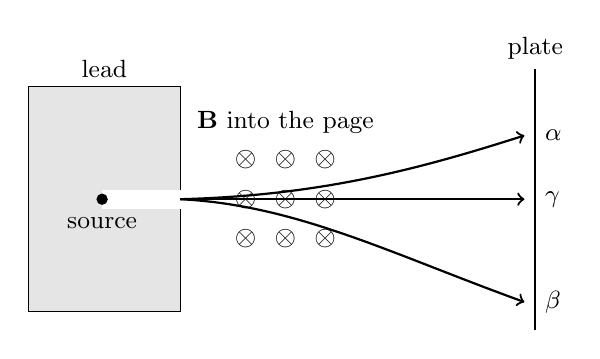
\begin{tikzpicture}[scale=0.92]
\draw[fill=gray!20] (0,-1.55) rectangle (2.1,1.55);
\draw[fill=white,draw=none] (1.02,-0.13) rectangle (2.12,0.13);
\draw[fill=black] (1.02,0) circle (0.07);
\node[below] at (1.02,-0.12) {\small source};
\node[above] at (1.05,1.55) {\small lead};
\foreach \x in {3.0,3.55,4.1}
  \foreach \y in {-0.55,0,0.55}
    \node at (\x,\y) {\(\otimes\)};
\node[above] at (3.55,0.78) {\small \(\mathbf B\) into the page};
\draw[thick] (7,-1.8) -- (7,1.8);
\node[above] at (7,1.8) {\small plate};
\draw[thick,->] (2.1,0) -- (6.85,0);
\draw[thick,->] (2.1,0) .. controls (4.0,0.05) and (5.35,0.40) .. (6.85,0.88);
\draw[thick,->] (2.1,0) .. controls (3.7,-0.08) and (5.0,-0.75) .. (6.85,-1.42);
\node[right] at (7,0.88) {\small \(\alpha\)};
\node[right] at (7,0) {\small \(\gamma\)};
\node[right] at (7,-1.42) {\small \(\beta\)};
\end{tikzpicture}
\caption{Коллимированный радиоактивный пучок в поперечном магнитном поле. Нейтральная компонента не отклоняется, тогда как противоположно заряженные компоненты изгибаются в противоположные стороны на разные величины.}
\end{figure}

Этим трём компонентам дали названия альфа, бета и гамма. В современных терминах,
\begin{equation}
\begin{aligned}
\beta\text{-radiation} &= \text{electrons},\\
\alpha\text{-radiation} &= \text{helium nuclei},\\
\gamma\text{-radiation} &= \text{photons}.
\end{aligned}
\end{equation}
Альфа-частица содержит два протона и два нейтрона, что объясняет её массовое число, равное четырём. В приблизительной целочисленной последовательности Дальтона гелий поэтому занимал бы место номер четыре: четыре ядерные единицы водородного масштаба. Бета-лучи — это отрицательно заряженные электроны, уже известные по экспериментам с катодными лучами. Гамма-лучи не несут электрического заряда.

При достаточно разреженном источнике и детекторе, способном различать отдельные приходы, непрерывный на вид след превращается в последовательность отдельных событий: щёлк, щёлк, щёлк. То же самое можно сделать для бета-, альфа- и гамма-излучения. Счётчик Гейгера даёт правильную картину, независимо от того, работали ли самые ранние установки точно в таком режиме. Каждая компонента приходит дискретными порциями. Гамма-излучение остаётся загадкой: оно нейтрально, однако регистрируется по одному событию за раз. Гамма-излучение — это свет очень высокой энергии, и Планк, а в особенности Эйнштейн, связали свет с квантами. Однако прежде чем подойти к этому выводу, нужно всерьёз отнестись к классическим свидетельствам того, что свет является волной.

\section{Классическая волновая природа света}

В классической физике свет был самым убедительным примером непрерывности. Он состоит из электрического и магнитного полей, распространяющихся как непрерывные волны. Ньютон отдавал предпочтение корпускулярной картине, но волновые эксперименты вытеснили её. Колебание заряда порождает электромагнитное излучение. Макроскопическая антенна может излучать радиоволны, микроволны, инфракрасное излучение, видимый свет или ультрафиолетовое излучение; заряд, движущийся внутри атома, тоже является антенной. Испущенное излучение может засветить фотографическую пластинку.

Одно отверстие даёт первое указание на волновое поведение. Если бы свет был потоком пуль, можно было бы ожидать, что маленькое отверстие создаст резко коллимированное пятно. Вместо этого освещённость расплывается в размытую область. Однако одного такого расплывания недостаточно для решающего вывода, потому что можно вообразить, что частицы отклоняются силами у края апертуры.

Два отверстия дают более резкую проверку. Два независимых потока частиц дали бы два перекрывающихся размытых пятна, возможно наиболее ярких там, где они перекрываются. Волны ведут себя иначе. Гребень из одного отверстия может встретиться с гребнем из другого, и тогда они усиливают друг друга; гребень может также встретиться с впадиной, и тогда они гасят друг друга. Поэтому на экране видны чередующиеся светлые и тёмные полосы, включая тёмные места, которые каждое из отверстий по отдельности освещало бы.\footnote{Схема воспроизводит диаграммы апертуры и интерференции, построенные в видеолекции в промежутке между 00:25:00 и 00:29:49.}

\begin{figure}[h]
\centering
\resizebox{\linewidth}{!}{%
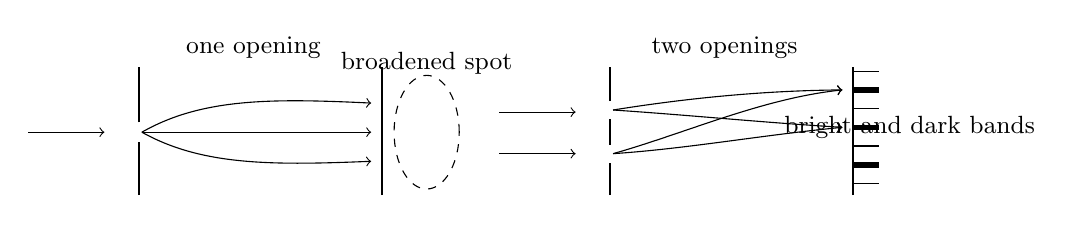
\begin{tikzpicture}[scale=0.88]
\begin{scope}
\draw[->] (-0.3,1.06) -- (0.8,1.06);
\draw[thick] (1.3,0.15) -- (1.3,0.92);
\draw[thick] (1.3,1.20) -- (1.3,2.0);
\draw[thick] (4.8,0.15) -- (4.8,2.0);
\draw[->] (1.34,1.06) .. controls (2.2,1.55) and (3.2,1.55) .. (4.65,1.48);
\draw[->] (1.34,1.06) -- (4.65,1.06);
\draw[->] (1.34,1.06) .. controls (2.2,0.58) and (3.2,0.58) .. (4.65,0.64);
\draw[dashed] (5.45,1.06) ellipse (0.47 and 0.82);
\node at (2.95,2.28) {\small one opening};
\node at (5.45,2.05) {\small broadened spot};
\end{scope}
\begin{scope}[xshift=6.8cm]
\draw[->] (-0.3,1.35) -- (0.8,1.35);
\draw[->] (-0.3,0.75) -- (0.8,0.75);
\draw[thick] (1.3,0.15) -- (1.3,0.62);
\draw[thick] (1.3,0.88) -- (1.3,1.25);
\draw[thick] (1.3,1.51) -- (1.3,2.0);
\draw[thick] (4.8,0.15) -- (4.8,2.0);
\draw[thin] (4.8,0.32) -- (5.18,0.32);
\draw[line width=2pt] (4.8,0.59) -- (5.18,0.59);
\draw[thin] (4.8,0.86) -- (5.18,0.86);
\draw[line width=2pt] (4.8,1.13) -- (5.18,1.13);
\draw[thin] (4.8,1.40) -- (5.18,1.40);
\draw[line width=2pt] (4.8,1.67) -- (5.18,1.67);
\draw[thin] (4.8,1.94) -- (5.18,1.94);
\draw[->] (1.34,0.75) .. controls (2.4,0.82) and (3.5,1.02) .. (4.65,1.13);
\draw[->] (1.34,1.38) .. controls (2.4,1.31) and (3.5,1.20) .. (4.65,1.13);
\draw[->] (1.34,0.75) .. controls (2.4,1.05) and (3.5,1.55) .. (4.65,1.67);
\draw[->] (1.34,1.38) .. controls (2.4,1.55) and (3.5,1.66) .. (4.65,1.67);
\node at (2.95,2.28) {\small two openings};
\node at (5.62,1.13) {\small bright and dark bands};
\end{scope}
\end{tikzpicture}
}
\caption{Одно отверстие создаёт уширенное изображение, тогда как два отверстия создают чередующиеся области конструктивной и деструктивной интерференции.}
\end{figure}

Тот же эффект нетрудно представить на воде. Пошевелите двумя пальцами на поверхности: круговые волны расходятся, в одних местах усиливают друг друга, а в других гасят. Решающим признаком волновой природы является именно интерференция, а не одно лишь распространение.

Историческая последовательность и здесь опять-таки не проста. В этой схематической версии изложения Huygens поставлен перед Newton как сторонник волнового распространения; Thomas Young связывается с демонстрацией интерференции; а некоторые собственные оптические эксперименты Newton допускают интерпретацию через волновую интерференцию, хотя он предпочитал корпускулы. Более поздние интерференционные эксперименты установили волновой характер света вне разумных сомнений.

Максвелл затем установил, что именно колеблется. Если световая волна распространяется вдоль некоторой оси, её электрическое поле поперечно к этой оси. Её магнитное поле тоже поперечно и перпендикулярно электрическому полю. Вся картина распространяется со скоростью света.\footnote{Схема воспроизводит диаграмму электромагнитной волны, нарисованную в видео лекции на отметке 00:31:08.}

\begin{figure}[h]
\centering
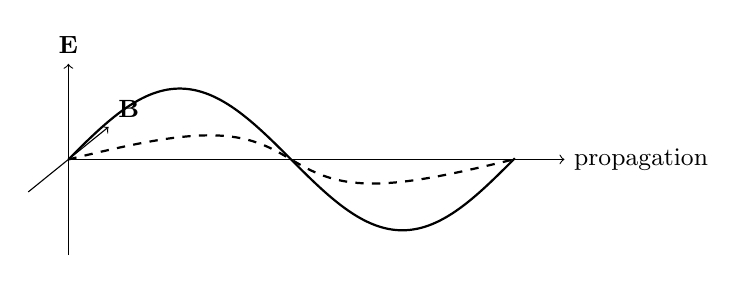
\begin{tikzpicture}[
  scale=0.9,
  x={(1cm,0cm)},
  y={(0cm,1cm)},
  z={(0.42cm,0.34cm)}
]
\draw[->] (0,0,0) -- (7,0,0) node[right] {\small propagation};
\draw[->] (0,-1.35,0) -- (0,1.35,0) node[above] {\small \(\mathbf E\)};
\draw[->] (0,0,-1.35) -- (0,0,1.35) node[above right] {\small \(\mathbf B\)};
\draw[thick,smooth,variable=\x,domain=0:6.3,samples=100]
  plot ({\x},{sin(\x r)},0);
\draw[thick,dashed,smooth,variable=\x,domain=0:6.3,samples=100]
  plot ({\x},0,{sin(\x r)});
\end{tikzpicture}
\caption{В электромагнитной волне электрическое и магнитное поля взаимно перпендикулярны и оба поперечны направлению распространения.}
\end{figure}

Обычный видимый свет колеблется слишком быстро, чтобы можно было непосредственно проследить чередующиеся поля. Для чрезвычайно длинной радиоволны колебание было бы соответственно более медленным. В обоих случаях интерференцию даёт одна и та же геометрия поперечной волны.

\section{Длина волны, период и частота}

Длина волны \(\lambda\) — это расстояние в пространстве: начните в некоторой точке колебания и двигайтесь вдоль волны, пока после одного полного цикла не повторится та же фаза. Она измеряется в метрах, сантиметрах или любой другой единице длины.

Теперь оставайтесь в одном месте, пока волна проходит мимо. Время, необходимое для одного полного цикла, есть период \(T\). Видимый свет имеет чрезвычайно короткий период, примерно порядка \(10^{-15}\,\mathrm{s}\); большей длине волны соответствует больший период, а меньшей длине волны — меньший период.

За один период волна проходит одну длину волны, поэтому для волны со скоростью \(v\) выполняется
\begin{equation}
v=\frac{\lambda}{T}.
\end{equation}
У водяных и звуковых волн свои скорости распространения. Для света
\begin{equation}
c=\frac{\lambda}{T}.
\end{equation}
Частота \(f\) — это число циклов в единицу времени:
\begin{equation}
f=\frac{1}{T}.
\end{equation}
Следовательно,
\begin{equation}
\lambda f=c.
\end{equation}
Каждая из этих величин определяет другую.

\begin{figure}[h]
\centering
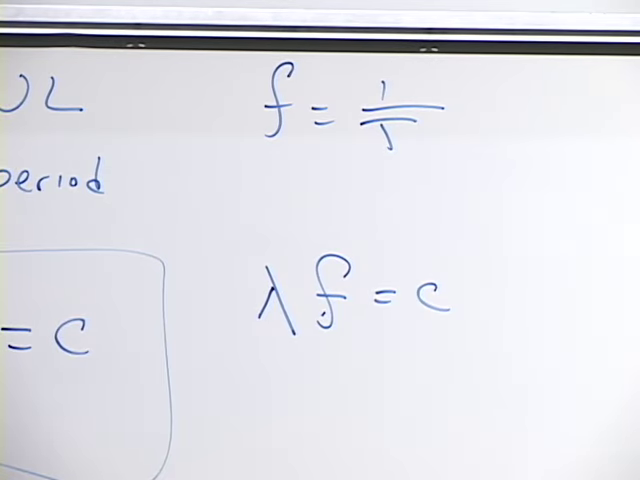
\includegraphics[width=0.68\textwidth]{lecture_01_figure_03.png}
\caption{Для световой волны \(f=1/T\) и \(\lambda f=c\).}
\lectureframe{00:36:24}
\end{figure}

Физики часто измеряют частоту колебаний в радианах в секунду, а не в полных циклах в секунду. Представьте себе равномерное движение по окружности. Если точка совершает \(f\) оборотов в секунду и каждый оборот содержит \(2\pi\) радиан, её угловая частота равна
\begin{equation}
\omega=2\pi f,
\qquad
\frac{\omega}{2\pi}=f.
\end{equation}
Пока что это определение; к практическому вопросу о том, уменьшает ли оно число множителей \(2\pi\), мы вернёмся позже.

Объединяя \(f=c/\lambda\) с \(\omega=2\pi f\), получаем
\begin{equation}
\omega=\frac{2\pi c}{\lambda},
\qquad
\omega\lambda=2\pi c.
\end{equation}
Для другого вида волны вместо \(c\) надо подставить её скорость распространения.

\begin{figure}[h]
\centering
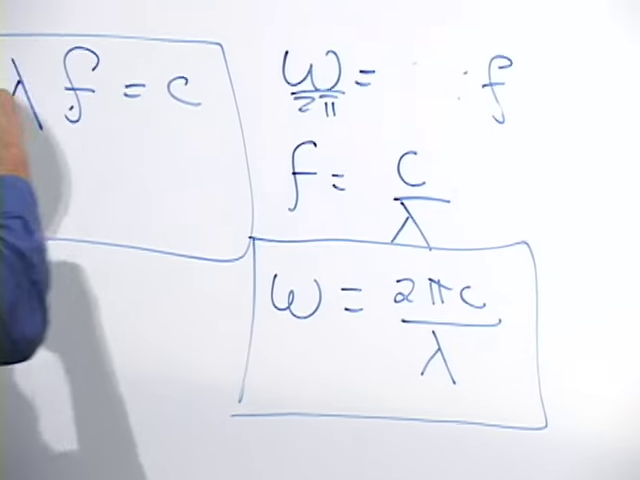
\includegraphics[width=0.68\textwidth]{lecture_01_figure_04.png}
\caption{Для световой волны при \(\omega=2\pi f\) выполняется \(\omega=2\pi c/\lambda\).}
\lectureframe{00:39:10}
\end{figure}

Электромагнитное излучение образует непрерывный спектр. Если упорядочить его от большей длины волны к меньшей, общепринятые названия таковы
\begin{equation}
\begin{aligned}
\text{radio}
&\longrightarrow \text{microwave}
\longrightarrow \text{infrared}
\longrightarrow \text{visible}\\
&\longrightarrow \text{ultraviolet}
\longrightarrow \text{X ray}
\longrightarrow \text{gamma ray}.
\end{aligned}
\end{equation}
Видимый свет занимает лишь узкий интервал. Границы между названными областями условны, поэтому точные разделяющие длины волн здесь не нужны. Радиоволны могут быть чрезвычайно длинными; гамма-излучение составляет самый коротковолновый конец электромагнитного спектра. Теперь трудность выступает особенно резко: гамма-излучение классически является непрерывной волной поля, однако регистрируется дискретными всплесками.

\section{Дискретные попадания и вероятности, задаваемые волной}

Термодинамические свойства излучения привели Planck и Einstein к выводу, что свет нужно рассматривать как состоящий из дискретных единиц. Воображаемый эксперимент делает эту мысль наглядной, но это не утверждение о действительном историческом пути к открытию.

Направьте пучок на экран. При обычной интенсивности он создаёт непрерывно выглядящее светлое пятно. Поместите в пучок частично непрозрачный аттенюатор: пятно станет тусклее. Снова и снова увеличивайте ослабление, и за единицу времени будет приходить всё меньше света. В конце концов картина изменится. Вместо непрерывно тусклого пятна детектор будет регистрировать отдельные события.\footnote{Схема воспроизводит эксперимент с ослаблением, разобранный в видео лекции между 00:42:32 и 00:45:42.}

\begin{figure}[h]
\centering
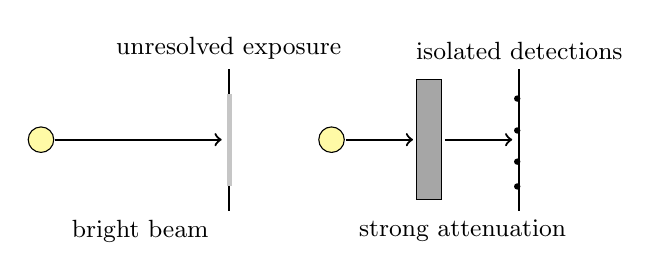
\begin{tikzpicture}[scale=0.9]
\begin{scope}
\draw[fill=yellow!35] (0,0) circle (0.18);
\draw[->,thick] (0.2,0) -- (2.55,0);
\draw[thick] (2.65,-1.0) -- (2.65,1.0);
\node[below] at (1.4,-1.0) {\small bright beam};
\end{scope}
\begin{scope}[xshift=4.1cm]
\draw[fill=yellow!35] (0,0) circle (0.18);
\draw[->,thick] (0.2,0) -- (1.15,0);
\draw[fill=gray!70] (1.2,-0.85) rectangle (1.55,0.85);
\draw[->,thick] (1.6,0) -- (2.55,0);
\draw[thick] (2.65,-1.0) -- (2.65,1.0);
\node[below] at (1.85,-1.0) {\small strong attenuation};
\end{scope}
\fill[gray!45] (2.62,-0.65) rectangle (2.70,0.65);
\foreach \y in {-0.66,-0.31,0.13,0.58}
  \fill (6.72,\y) circle (0.045);
\node[above] at (2.65,1.0) {\small unresolved exposure};
\node[above] at (6.75,1.0) {\small isolated detections};
\end{tikzpicture}
\caption{Постепенное ослабление уменьшает частоту регистрации, пока непрерывно выглядящая экспозиция не распадается на отдельные фотонные события.}
\end{figure}

Если подождать достаточно долго, эти события накопятся в тот же пространственный профиль, что и исходное пятно. Значит, яркая область была неразрешённой суммой многих отдельных попаданий. Такой эксперимент при малой интенсивности можно провести, хотя это не тот ранний эксперимент, который первоначально побудил к фотонной гипотезе. Предложение Einstein о фотоне возникло из термодинамических и фотоэлектрических соображений; эксперимент с ослаблением даёт особенно прямой способ представить его следствие.

Теперь поместите в пучок два отверстия и уменьшите интенсивность так, чтобы фотоны приходили по одному. Каждая регистрация — это локализованный всплеск. И всё же после многих регистраций эти всплески заполняют интерференционную картину, включая светлые и тёмные полосы. Дискретные попадания случайны, но их распределение вероятностей совпадает с распределением, предсказываемым волновой картиной. Классическая волна превратилась в волну, задающую вероятности.

Следовательно, волна и частица — не два отдельных типа сущностей, приписываемых разным частям природы. Это два проявления одного и того же квантового объекта. Свет нельзя адекватно описать ни только как волну, ни только как частицу.

С электронами исходное удивление обращается вспять. Электроны считались частицами и приходят на детектор по одному, но при достаточно близко расположенных отверстиях они тоже образуют интерференционную картину. Альфа-частицы, примерно в 8000 раз тяжелее электронов, подчиняются тому же принципу, хотя эксперимент труднее. Интерференция наблюдалась даже для бакиболов: молекул из 60 атомов углерода, расположенных приблизительно как обобщённый футбольный мяч. Ожидается, что тот же принцип применим даже к шарам для боулинга, хотя такой эксперимент фантастически непрактичен. Можно пойти ещё дальше и рассматривать предлагаемые эксперименты с вирусами или живыми клетками как всё более смелые примеры. Понимание того, как согласуются волновое и корпускулярное описания, требует квантовой механики; непосредственная задача сейчас — выделить свойства фотона, нужные для физики элементарных частиц.

\section{Энергия фотона}

Фотоны — дискретные, неделимые элементы света. Свет несёт энергию---солнечный свет нагревает поглощающее тело---поэтому каждый фотон должен нести энергию. Монохроматическая волна имеет определённые длину волны и угловую частоту, и каждый фотон в ней имеет
\begin{equation}
E_\gamma=\hbar\omega.
\end{equation}
Пытаться представлять непрерывную волну как маленькое механическое скопление точек — значит вводить в заблуждение. Определённым является экспериментальное сочетание: локализованные регистрации происходят с распределением, задаваемым волной, а энергия приходит неделимыми порциями.

Поскольку
\begin{equation}
\omega=\frac{2\pi c}{\lambda},
\end{equation}
меньшая длина волны означает большую угловую частоту и, следовательно, большую энергию каждого фотона:
\begin{equation}
\lambda\downarrow
\quad\Longrightarrow\quad
\omega\uparrow
\quad\Longrightarrow\quad
E_\gamma\uparrow.
\end{equation}
Один фотон радиодиапазона имеет очень малую энергию. Тем не менее радиопучок может нести огромную полную энергию, если он содержит очень много фотонов. Для монохроматического импульса, содержащего \(n\) фотонов,
\begin{equation}
E_{\text{pulse}}=n\hbar\omega,
\qquad
n=0,1,2,\ldots.
\end{equation}
Полная энергия может быть большой, но она остаётся целым кратным энергии одного фотона.

Это соотношение подводит к практическому вопросу, который будет определять всё дальнейшее обсуждение. Почему, чтобы увидеть всё меньшие и меньшие объекты, приходится строить всё большие и большие машины? Почему не использовать маленькую машину для маленького объекта? Первая половина ответа уже налицо: чтобы разрешить более мелкую структуру, нужна меньшая длина волны, а квант с меньшей длиной волны несёт большую энергию.

\section{Энергия покоя и инвариантная масса}

Физика элементарных частиц объединяет квантовую механику и теорию относительности. Соответствующей квантовой стороной служит соотношение для фотона \(E_\gamma=\hbar\omega\); соответствующим элементарным фактом со стороны теории относительности является
\begin{equation}
E_{\mathrm{rest}}=mc^2.
\end{equation}
Это уточнение существенно. В старых изложениях различали \emph{массу покоя} и зависящую от скорости \emph{движущуюся массу}. В современной терминологии \emph{масса} означает инвариантную массу объекта. Движение изменяет его энергию, а не массу. У каждого электрона одна и та же масса, в каком бы состоянии движения он ни находился, тогда как энергия электрона возрастает по мере его ускорения. Следовательно, \(E=mc^2\) в этой форме есть энергия массивного объекта в системе отсчёта, в которой объект как целое покоится.

Объект не обязан быть внутренне неподвижным. Ящик с газом может неподвижно стоять на весах, тогда как его молекулы быстро движутся во всех направлениях. Энергия этих внутренних движений входит в энергию покоя всего ящика. Если начать с холодного ящика, измерить его массу, а затем добавить тепловую энергию, удерживая сам ящик в покое, то его масса покоя изменится на
\begin{equation}
\Delta m=\frac{\Delta E_{\mathrm{internal}}}{c^2}.
\end{equation}
Его вес и инерция увеличиваются вместе с массой. Для обычного ящика даже после сильного повышения температуры эффект слишком мал, чтобы заметить его на обычных весах; малость эффекта не меняет самого принципа.

Более наглядный пример связан с электроном и позитроном. У них в точности равные массы и противоположные электрические заряды. Если они изначально покоятся и аннигилируют, фотоны уносят энергию:
\begin{equation}
e^-+e^+\longrightarrow \text{photons}.
\end{equation}
Начальная энергия равна
\begin{equation}
E_{\mathrm{initial}}=2m_e c^2,
\end{equation}
и эта энергия не может исчезнуть. Одна пара даёт лишь очень малую энергию, так что, чтобы нагреть хотя бы чашку кофе, потребовались бы огромные числа пар, но отдельные акты аннигиляции непосредственно демонстрируют это превращение.

Для покоящегося объекта масса и энергия, следовательно, являются одной и той же физической величиной, выраженной в разных единицах. Множитель \(c^2\) служит коэффициентом перевода между обычными единицами массы и энергии, подобно тому как численный множитель переводит метры в сантиметры.

\begin{classroomqa}
\lecturetimestamp{01:04:39}
\audiencequestion{Требуется ли механизм для превращения массы в высвобождаемую энергию?}
\lecturerresponse{Да, физический механизм требуется, но законы сохранения уже ограничивают результат. Ещё до описания микроскопического механизма аннигиляции начальная энергия электрон--позитронной пары должна где-то вновь появиться. Поэтому закон сохранения энергии позволяет установить важную часть ответа и без подробного описания взаимодействия.}
\end{classroomqa}

\section{Размерности и выбор единиц}

В единицах СИ скорость света — очень большое число, а постоянная Планка — очень маленькое. На малость последней уже указывает фотонное соотношение: угловая частота видимого света огромна, тогда как энергия одного фотона ничтожна, так что \(E_\gamma=\hbar\omega\) требует малого численного значения \(\hbar\) в этих единицах. По порядку величины,
\begin{equation}
c\sim 10^8\ \mathrm{m\,s^{-1}},
\qquad
\hbar\sim 10^{-34}\ \mathrm{J\,s}.
\end{equation}
\editorialnote{Сохранены только порядки величин, указанные на лекции, поскольку последние цифры на доске неразличимы.}
Единицы существенны: ни одна из этих констант не является просто числом без единиц. Поскольку энергия имеет размерность
\begin{equation}
[E]=M L^2 T^{-2},
\end{equation}
а \(E_\gamma=\hbar\omega\) при \([\omega]=T^{-1}\), постоянная Планка имеет размерность
\begin{equation}
[\hbar]=[E]T=M L^2 T^{-1}.
\end{equation}

Называть \(c\) большой, а \(\hbar\) малой — уже значит предполагать выбор единиц. Измерение скорости в футах в час даёт другое численное значение \(c\), чем измерение в метрах в секунду. В световых годах в год, или в световых секундах в секунду, скорость света просто равна единице. Точно так же подходящий согласованный выбор единиц массы, длины и времени может привести к тому, что \(\hbar=1\).

Привычные системы единиц — это унаследованные соглашения, а не привилегированные свойства природы. В миле 5280 футов, в стоуне 14 фунтов, рост лошадей измеряют в ладонях, а мощность можно измерять в лошадиных силах. Метрические единицы более систематичны, но их масштабы всё равно выбраны людьми. Ничто в фундаментальной физике не выделяет метр, секунду или килограмм.

Длина, время и масса задают три независимых выбора основных единиц:
\begin{equation}
L,\qquad T,\qquad M.
\end{equation}
Из них можно построить другие механические единицы. Полезный выбор зависит от задачи. Солнечная масса удобна в астрофизике; масса протона может быть удобна в ядерной физике; световые годы и годы делают релятивистские астрономические формулы компактными. Имея три независимых выбора, можно задать удобные численные значения трём независимым размерным константам. Астрофизика, атомная физика и физика элементарных частиц не обязаны делать один и тот же выбор.

Для физики элементарных частиц особенно полезны два соглашения
\begin{equation}
c=1,
\qquad
\hbar=1.
\end{equation}
Для оставшейся единицы нет столь же выделенной массы частицы. Можно было бы объявить равной единице массу протона, массу бозона Хиггса или массу мюона, но это лишь выделило бы один объект из большого множества.

Почему тогда выбирают \(c\) и \(\hbar\)? Первым ответом могло бы быть то, что они входят во многие уравнения. Частота появления недостаточна: масса протона тоже входит во многие уравнения, и размер протона тоже. То, что отличает \(c\) и \(\hbar\), — это их универсальность.

Константы \(c\) и \(\hbar\) имеют иной характер. Скорость \(c\) ограничивает любой физический объект: массивные объекты могут к ней приближаться, но не могут быть разогнаны до скоростей выше неё. Постоянная Планка ограничивает любой квантовый объект через соотношение неопределённостей по порядку величины
\begin{equation}
\Delta x\,\Delta p\gtrsim\hbar.
\end{equation}
Ни одно из этих утверждений не выделяет какой-то конкретный вид частицы. Именно эта универсальность делает \(c=1\) и \(\hbar=1\) естественными соглашениями.

Протон не задаёт сопоставимого универсального масштаба. Он лишь один объект среди многих. Приравнивание массы протона к единице не имело бы большего фундаментального статуса, чем приравнивание к единице массы атома рубидия; с электроном, бозоном Хиггса и мюоном возникает та же трудность.

Электрический заряд подсказывает ещё одну универсальную величину, но после нормировки \(c\) и \(\hbar\) физически существенная электромагнитная константа связи оказывается безразмерной. Изменение единиц может перераспределять размерные константы в электромагнитной формуле; изменить подлинную безразмерную константу связи оно не может.

Гравитация даёт универсальную размерную константу. В ньютоновской форме модуль силы между двумя массами равен
\begin{equation}
F=G\frac{m_1m_2}{r^2}.
\end{equation}
Любая масса гравитирует, тогда как электрически нейтральные объекты не обязаны испытывать электрическую силу. Следовательно, \(G\) обладает требуемой универсальностью. Тем не менее для обычной физики элементарных частиц это плохой практический выбор нормировки, потому что гравитационные силы между известными элементарными частицами пренебрежимо малы в обсуждаемых вычислениях.

\begin{classroomqa}
\lecturetimestamp{01:20:34}
\audiencequestion{Допустимо ли просто отбросить \(G\)? При очень высоких энергиях элементарные частицы могут не подчиняться классической гравитации в предполагаемом здесь виде.}
\lecturerresponse{Отдельные частицы действительно реагируют на гравитационное поле Земли: одиночная частица падает в этом поле. Гравитационное влияние одной элементарной частицы на другую напрямую не измерялось, так что предположение об универсальности на этом уровне можно поставить под вопрос. Непосредственная причина не включать \(G\) скорее практическая, чем абсолютная: вклад гравитации в обычные эксперименты и уравнения физики элементарных частиц пренебрежимо мал.}
\end{classroomqa}

\begin{classroomqa}
\lecturetimestamp{01:22:01}
\audiencequestion{Можно ли использовать электрическое взаимодействие как третье соглашение о выборе единиц вместо гравитации?}
\lecturerresponse{Да. Можно выбрать электромагнитные единицы, в которых нормирован электрический заряд или константа, входящая в закон Кулона. Такие соглашения используются. Электроны отталкиваются, а не притягиваются, но этот знак не мешает такому выбору. Просто здесь принято не это соглашение.}
\end{classroomqa}

\begin{classroomqa}
\lecturetimestamp{01:23:06}
\audiencequestion{После того как \(c\) и \(\hbar\) приравнены к единице, является ли электрический заряд безразмерным?}
\lecturerresponse{Да. Безразмерная величина, связанная с квадратом электрического заряда, приблизительно равна \(1/137\). Точное соглашение и смысл этого числа можно пока оставить в стороне; здесь важно лишь то, что оно безразмерно.}
\end{classroomqa}

\begin{classroomqa}
\lecturetimestamp{01:23:37}
\audiencequestion{Можно ли выбрать постоянную Кулона в качестве третьей константы, приравниваемой к единице?}
\lecturerresponse{Её можно поглотить выбором электромагнитных единиц. Этот выбор не может превратить безразмерную константу связи \(1/137\) в единицу, потому что изменение единиц не может изменить безразмерное число. Здесь не утверждается, что принятие такого соглашения даёт какое-либо особое преимущество.}
\end{classroomqa}

\section{Уравнения в естественных единицах и системы отсчёта}

При \(c=1\) соотношение для энергии покоя массивного объекта принимает вид
\begin{equation}
E_{\mathrm{rest}}=m.
\end{equation}
При \(\hbar=1\) соотношение для фотона принимает вид
\begin{equation}
E_\gamma=\omega.
\end{equation}
Если нужны численные значения в обычных единицах, эти константы всегда можно восстановить.

\begin{figure}[h]
\centering
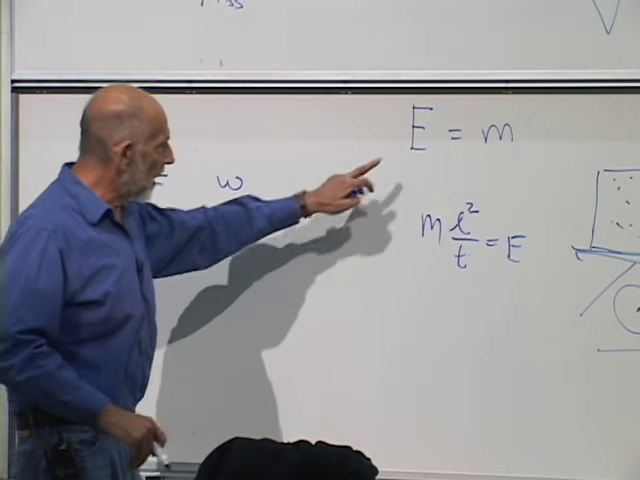
\includegraphics[width=0.72\textwidth]{lecture_01_figure_05.png}
\caption{В единицах, где \(c=1\), энергия покоя объекта с массой, находящегося в покое, равна \(E=m\).}
\lectureframe{01:25:40}
\end{figure}

Эти формулы выглядят похоже, но означают разное. В \(E_{\mathrm{rest}}=m\) \(E\) — энергия покоя объекта с массой. Фотон не имеет массы и не может быть приведён в состояние покоя, поэтому его энергия не является энергией покоя. Соотношение \(E_\gamma=\omega\) задаёт энергию движущегося безмассового кванта.

\begin{classroomqa}
\lecturetimestamp{01:26:07}
\audiencequestion{Что означает \emph{«в покое»}, если покой всегда относителен к чему-то и сама лаборатория не находится в абсолютном покое?}
\lecturerresponse{Покой определяется относительно выбранной системы отсчёта. Если чашка покоится относительно лаборатории, то в этой лабораторной системе отсчёта её энергия при \(c=1\) равна её массе, без какого-либо суммарного кинетического вклада. Другой наблюдатель, движущийся мимо чашки, припишет ей также кинетическую энергию. Разные наблюдатели, вообще говоря, приписывают одному и тому же объекту или фотону разные энергии; энергия зависит от системы отсчёта, и никакого утверждения об абсолютном покое не требуется.}
\end{classroomqa}

Теперь можно снова вернуться к соглашению об угловой частоте. Запись \(E_\gamma=\hbar\omega\) компактна, но соотношение \(\omega=2\pi f\) ранее внесло множитель \(2\pi\).

\begin{classroomqa}
\lecturetimestamp{01:28:13}
\audiencequestion{Почему используют угловую частоту \(\omega\), измеряемую в радианах в секунду, а не, казалось бы, более простое число полных циклов в секунду?}
\lecturerresponse{Этот выбор отчасти исторический, а математический ответ здесь скорее прагматический, чем прямой. Предлагаемый здесь ответ предварителен: запишите соответствующие уравнения один раз с \(f\) и один раз с \(\omega\), а затем посмотрите, при каком соглашении остаётся меньше множителей \(2\pi\). От множителей \(2\pi\) невозможно избавиться всюду. Также была упомянута возможная связь с записью через комплексную экспоненту, но здесь она не развивается.}
\end{classroomqa}

\begin{classroomqa}
\lecturetimestamp{01:29:51}
\audiencequestion{Можно ли разогнать две частицы до тех пор, пока их взаимное гравитационное взаимодействие не станет существенным?}
\lecturerresponse{В принципе да. На практике современные ускорители чрезвычайно далеки от этого режима. Ответ также зависит от того, что имеется в виду под частицей: макроскопическое гравитирующее тело — не тот случай элементарных частиц, о котором идёт речь.}
\end{classroomqa}

\begin{classroomqa}
\lecturetimestamp{01:30:27}
\audiencequestion{Что может быть источником позитронов?}
\lecturerresponse{Высокоэнергичные столкновения могут рождать позитроны. Некоторые ядерные процессы и распады тоже их порождают.}
\end{classroomqa}

\begin{classroomqa}
\lecturetimestamp{01:30:53}
\audiencequestion{Являются ли планковское время и планковская длина теми естественными единицами, которые здесь используются?}
\lecturerresponse{Нет. Планковские единицы возникают, когда \(G\), \(c\) и \(\hbar\) все полагаются равными единице. Получающаяся планковская длина намного меньше характерных масштабов длины в обычной физике элементарных частиц, поэтому здесь она неудобна как единица измерения. Такие единицы естественны, когда одновременно существенны гравитация, квантовая механика и теория относительности, как в физике чёрных дыр, космологии или квантовой гравитации. Когда гравитацией можно пренебречь, полезнее полагать равными единице только \(c\) и \(\hbar\).}
\end{classroomqa}

\section{Импульс, свет и разрешение}

Следующее основное понятие — импульс. Объект в покое не имеет импульса, хотя обладает ненулевой энергией покоя \(mc^2\). Как только он начинает двигаться, он, вообще говоря, несёт импульс. Импульс сохраняется при столкновении так же, как сохраняется энергия: когда сталкиваются два объекта, полный векторный импульс до и после столкновения одинаков. Всякая величина, подчиняющаяся закону сохранения, заслуживает особого внимания.

Импульс — вектор: он направлен вдоль движения. Для нерелятивистского объекта,
\begin{equation}
\mathbf p=m\mathbf v.
\end{equation}
Это не общая релятивистская формула, и непосредственно к свету её применять нельзя.

Свет, тем не менее, переносит не только энергию, но и импульс. Обычный свет создаёт настолько малый толчок, что заметить его импульс трудно, но интенсивный лазерный импульс может передать существенный механический толчок. Например, крупный лазер в Livermore может вдавливать вещество внутрь благодаря импульсу, переносимому его излучением.

Рассмотрим световой импульс, достаточно хорошо коллимированный, чтобы его лучи шли почти вдоль одной оси. У реального пучка может быть некоторый угловой разброс, так что отдельные его части распространяются в немного разных направлениях, но для идеального коллимированного пучка импульс направлен вдоль пучка и имеет величину
\begin{equation}
p=\frac{E}{c},
\qquad\text{or equivalently}\qquad
E=cp.
\end{equation}
Это соотношение здесь принимается как релятивистский факт, а не выводится. Следующая проверка размерностей лишь подтверждает, что его единицы совпадают с единицами обычного импульса:
\begin{equation}
\left[\frac{E}{c}\right]
=
\frac{M L^2 T^{-2}}{L T^{-1}}
=
M L T^{-1}
=
[m v]
=
[p].
\end{equation}
Это сравнение размерностей не приписывает свету массу покоя. Фотон имеет нулевую массу; он несёт импульс потому, что несёт энергию и движется со скоростью \(c\).

Направление \(\mathbf p\) совпадает с направлением распространения. Его модуль обычно трудно обнаружить, потому что в знаменателе стоит \(c\). Пучок может легко проявить свою энергию, нагревая или испаряя вещество, тогда как его механический толчок гораздо меньше. Однако при достаточно большой интенсивности этот толчок может стать значительным.

Для одного фотона,
\begin{align}
p_\gamma
&=\frac{E_\gamma}{c}\\
&=\frac{\hbar\omega}{c}.
\end{align}
Чтобы выразить это через длину волны, аккуратно вернёмся к волновым соотношениям. Поскольку
\begin{equation}
f\lambda=c,
\qquad
\omega=2\pi f,
\end{equation}
правильное соотношение имеет вид
\begin{equation}
\omega\lambda=2\pi c,
\qquad
\omega=\frac{2\pi c}{\lambda}.
\end{equation}
С множителем \(2\pi\) легко по ошибке обратить всё наоборот, если не выписать определения. Если заново исходить из \(f\lambda=c\) и \(f=\omega/(2\pi)\), вопрос снимается:
\begin{equation}
\frac{\omega}{2\pi}\lambda=c
\quad\Longrightarrow\quad
\omega\lambda=2\pi c.
\end{equation}
Подстановка теперь даёт
\begin{align}
p_\gamma
&=\frac{\hbar}{c}\frac{2\pi c}{\lambda}\\
&=\frac{2\pi\hbar}{\lambda}\\
&=\frac{h}{\lambda}.
\end{align}

\begin{classroomqa}
\lecturetimestamp{01:42:38}
\audiencequestion{Равно ли \(2\pi\hbar\) величине \(h\)?}
\lecturerresponse{Да. По определению \(h=2\pi\hbar\), так что \(p_\gamma=2\pi\hbar/\lambda\) — то же самое, что и \(p_\gamma=h/\lambda\). Множители \(2\pi\) где-то вновь появляются при любом выборе соглашения о частоте.}
\end{classroomqa}

Чем короче длина волны, тем больше импульс фотона. Радиофотон имеет очень большую длину волны и крошечный импульс. Фотон гамма-излучения имеет очень короткую длину волны и сообщает гораздо более сильный толчок. Один фотон всё равно даёт лишь малый макроскопический толчок, но его импульс намного больше, чем у радиофотона. Его энергия также больше, поскольку \(E_\gamma=cp_\gamma\).

Это соотношение объясняет, почему меньшие объекты требуют более крупных установок. Фотография, полученная при длинах волн, намного больших, чем голова человека, могла бы показать лишь размытое пятно. Чтобы различить черты лица, длина волны должна быть меньше размера головы. Чтобы разрешить один волос, она должна быть сравнима с толщиной волоса или меньше неё. Чтобы разрешить структуру атома, длина волны зонда должна быть не больше самого атома:
\begin{equation}
\lambda_{\mathrm{probe}}\lesssim
\text{size of the structure to be resolved}.
\end{equation}
Следовательно, меньшие структуры требуют более коротких длин волн, а более короткие длины волн требуют большего импульса и энергии. Зонд не обязательно должен быть фотоном; высокоэнергетические частицы других видов подчиняются той же квантовой связи между длиной волны и импульсом. Для их получения нужны ускорители, которые передают каждой частице всё больше и больше энергии. Аргумент опирается на пару \(p_\gamma=h/\lambda\) и \(E_\gamma=\hbar\omega\): увеличение энергии зонда увеличивает его импульс и укорачивает его длину волны.

Такова повторяющаяся картина физики элементарных частиц уже примерно столетие: выше энергия, больше импульс, короче длина волны и выше пространственное разрешение.

\begin{classroomqa}
\lecturetimestamp{01:46:57}
\audiencequestion{Есть ли теоретический нижний предел длины волны?}
\lecturerresponse{Возможно. Вблизи планковской длины ожидается нечто новое, но ответ пока предварителен. Если пространственное разрешение достигает там нижнего предела, то этот масштаб всё равно примерно на 17 порядков меньше расстояний, зондируемых на LHC, так что современные эксперименты остаются от него чрезвычайно далеки.}
\end{classroomqa}

Та же цепочка рассуждений указывает на грубую связь между масштабом ускорителя и масштабом, который он может разрешить.

\begin{classroomqa}
\lecturetimestamp{01:48:02}
\audiencequestion{Находятся ли длина волны, или разрешаемый размер, приблизительно в обратной зависимости от размера ускорителя?}
\lecturerresponse{Приблизительно да, если максимальные электрические поля, ускоряющие частицы, и магнитные поля, используемые для их направления, фиксированы возможностями имеющейся аппаратуры. Ускоряющий градиент — это прирост энергии на единицу длины. Для линейного ускорителя длины \(L\) и приблизительно фиксированного градиента \(\mathcal G\),
\[
E_{\mathrm{beam}}\sim \mathcal G L.
\]
При ультрарелятивистских энергиях разрешаемая длина волны обратно связана с энергией, поэтому увеличение длины линейного ускорителя улучшает разрешение примерно в той же обратной пропорции. Это лишь эвристическое масштабирование, а не точный закон. В кольцевых машинах одну и ту же установку можно проходить многократно, но ускоренные заряды при искривлении траектории излучают и теряют энергию.}
\end{classroomqa}

\begin{classroomqa}
\lecturetimestamp{01:49:47}
\audiencequestion{Насколько большим должен был бы быть ускоритель, чтобы достичь планковской длины?}
\lecturerresponse{При таком грубом масштабировании он должен был бы быть примерно на 17 порядков длиннее ускорителя CERN. Это не размер Вселенной, но по масштабу он был бы примерно галактическим.}
\end{classroomqa}

\begin{classroomqa}
\lecturetimestamp{01:50:09}
\audiencequestion{Как соотносятся энергии космических лучей наивысших энергий с энергиями коллайдеров?}
\lecturerresponse{Отдельные космические лучи могут иметь гораздо большую лабораторную энергию. Для численного сравнения возьмём экстремальный космический луч с лабораторной энергией порядка \(10^{21}\,\mathrm{eV}=10^{12}\,\mathrm{GeV}\). Но космический луч сталкивается с мишенью, покоящейся в лабораторной системе, тогда как в коллайдере два энергичных пучка сводятся лоб в лоб. Ещё важнее то, что для содержательных экспериментов требуется поток: много частиц и много хорошо контролируемых столкновений. Одиночный космический луч может не попасть в нужную мишень или породить событие, по которому мало что можно заключить. Намеренно экстравагантная оценка в нефтяном эквиваленте даёт для обеспечения работы галактического ускорителя, пригодного для таких экспериментов, около ста триллионов баррелей нефти в секунду. Её цель — показать, что достаточная статистика столкновений была бы по меньшей мере столь же серьёзным препятствием, как и длина ускорителя.}
\end{classroomqa}

\editorialnote{Оценка в нефтяном эквиваленте в источнике непоследовательна. Сначала она приводится, а затем повторяется как приблизительно \(10^{14}\) баррелей в секунду; в более позднем повторном изложении указано \(10^{11}\) баррелей в секунду. Оба масштаба сохранены, а не молча согласованы.}

Это реальные масштабы расстояний, а не просто формальные. Практическая проблема состоит в том, как зондировать их, не строя галактический ускоритель и не обеспечивая его фантастической мощностью.

\begin{classroomqa}
\lecturetimestamp{01:52:55}
\audiencequestion{Как следует сопоставлять энергию LHC с энергией космического луча \(10^{12}\,\mathrm{GeV}\)?}
\lecturerresponse{Для ультрарелятивистской налетающей частицы с лабораторной энергией \(E_{\mathrm{lab}}\), сталкивающейся с неподвижной мишенью массы \(m_{\mathrm{target}}\), энергия в системе центра масс параметрически масштабируется как
\[
E_{\mathrm{cm}}\simeq
\sqrt{2m_{\mathrm{target}}c^2E_{\mathrm{lab}}}.
\]
\editorialnote{Приведённое выражение для неподвижной мишени явно показывает указанное в этом обмене репликами корневое масштабирование.}
При фиксированной массе мишени полезная энергия столкновения поэтому растёт лишь как квадратный корень из энергии налетающей частицы. Поэтому космический луч с энергией \(10^{12}\,\mathrm{GeV}\) соответствует, по порядку величины, энергиям встречных пучков порядка \(10^6\,\mathrm{GeV}\) на пучок, а не \(10^{12}\,\mathrm{GeV}\) в каждом пучке. Космические лучи всё же могут превосходить энергии земных коллайдеров, но их крайне малый поток делает систематические, контролируемые эксперименты непрактичными.}
\end{classroomqa}